As our goal is to achieve high re-usability, modularity and openness, we built our software architecture on the Robot Operating System (ROS) middleware, using version Indigo \cite{ros} running on Ubuntu Trusty Tahr. 
Additionally, our system this year uses some of the publicly released packages from the STRANDS project \cite{strands}. 
This allows us not only integrate the cutting edge research to our robot, but also contribute to the evaluation of this research. 
Moreover, we integrate our own research where our interest overlaps with the focus of the competition.
Our system architecture can be seen on Fig.~\ref{fig:architecture} containing six modules which are explained below.

\subsection{State machine}

Even though, AI planning is in our expertise, we use \textit{finite state machines} to control and monitor robot's states and actions. 
We have two main reasons for this decision. First, the competition defines all \textit{task benchmarks} as short scripts, so a robot does not have too much freedom in order to decide how to fulfil a task. Second, a state machine provides us with \textit{repeatability} during testing.

For each of the benchmarks, we develop the state machine using ROS's SMACH package, that is ``a task-level architecture for rapidly creating complex robot behaviour" \cite{smach}. 
All of the task's state machines are linked with the central state machine which communicates with the referee box. 


%\begin{figure}[!htb]
%\centering
%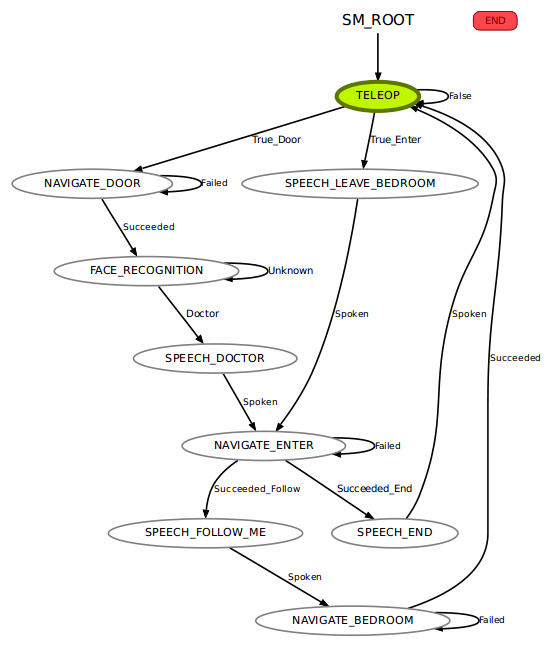
\includegraphics[width=3.in]{state_machine.png}
%\caption{SMACH state machine connecting all subsystems to one robotic framework}
%\label{fig:smach}
%\end{figure}

\subsection{Navigation}

\paragraph{Mapping} - we used \textit{OpenSlam's GMapping} algorithm \cite{slam} through the ROS wrapper package called \textsf{slam gmapping}. This approach uses a Rao-Blackwellized particle filter in which each particle carries an individual map of the environment. The particles are updated by taking into account both odometry and the latest observations from a laser range finder.

\paragraph{Localising} in a known map with Adaptive Monte Carlo Localisation.
After the map is known and saved, an \textit{Adaptive Monte Carlo Localisation} (AMCL)\cite{amcl} algorithm is used to localise the robot inside the known environment. This node is part of the ROS \textsf{navigation stack} package. For details, see the section below. It uses laser range finder readings to update a particle filter. Every particle represents a specific discrete state and stores the uncertainty of the robot being in that state/position within the known map. Also, every time the robot moves it uses the motor information to shift the particles to the corresponding direction.

\paragraph{Move-base} For navigation and obstacle avoidance, ROS's \textsf{navigation stack} is used. It is a proven robust solution for domestic environments \cite{Marder-Eppstein2010}. More specifically this node reads the odometry, the current pose estimate and the laser range finder scans from the relevant topics and safely drives the robot in the environment to a predefined goal. In order to navigate smoothly, it uses a combination of a global and a local planner. The global planner creates an optimal global path based on the robot's pose and a global cost-map. Then the local planner, which uses the \textit{Dynamic Window Approach} algorithm \cite{dwa}, is responsible for following the global path and reactively avoiding obstacles.


\subsection{Object detection and recognition}
%small vs big

\subsection{Human detection and interaction}

\paragraph{\label{sec:vision}Face detection and recognition}
In order to be able to recognise a person standing in front of the entrance, the system implements face detection, which is used to find candidate face patterns inside an image, and face recognition, which finds the best match of a detected face with a known dataset, see Fig. \ref{fig:face}.

Face detection is performed using the \textit{Viola-Jones} algorithm \cite{Viola01_RapidObjDet}. The algorithm looks for faces by applying incrementally many simple Haar classifiers. The composition is performed by a cascade function, which needs to be trained \textit{a priori} with many positive and negative images. The resulting classifier can find faces efficiently with independence of the size of the faces and light conditions.

Face recognition is performed by applying a \textit{Local Binary Pattern Histogram} (LBPH) algorithm \cite{Ahonen04_FaceRecLBP}. The principle of the algorithm is to build local binary patterns (LBP) for each pixel depending on a variable neighbourhood scheme. Then, it divides the formed LBP image into $m$ local regions and computes the LBP distribution histogram from each region. Finally, classification is performed by comparison between the LBP histograms of a new face with the ones from the dataset.

%\begin{figure}[!t]
%\centering
%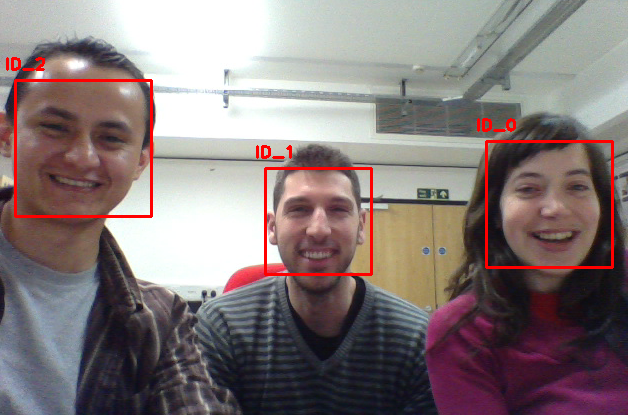
\includegraphics[width=3.in]{BARC_FaceRec.png}
%\caption{An example of the face detection and face recognition algorithms. The red bounding boxes surround the successfully detected faces, while each of them is given a corresponding identification code.}
%\label{fig:face}
%\end{figure}

\subsection{Speech recognition}

\subsection{Semantic mapping}



%\begin{figure*}[!t]
%\centering
%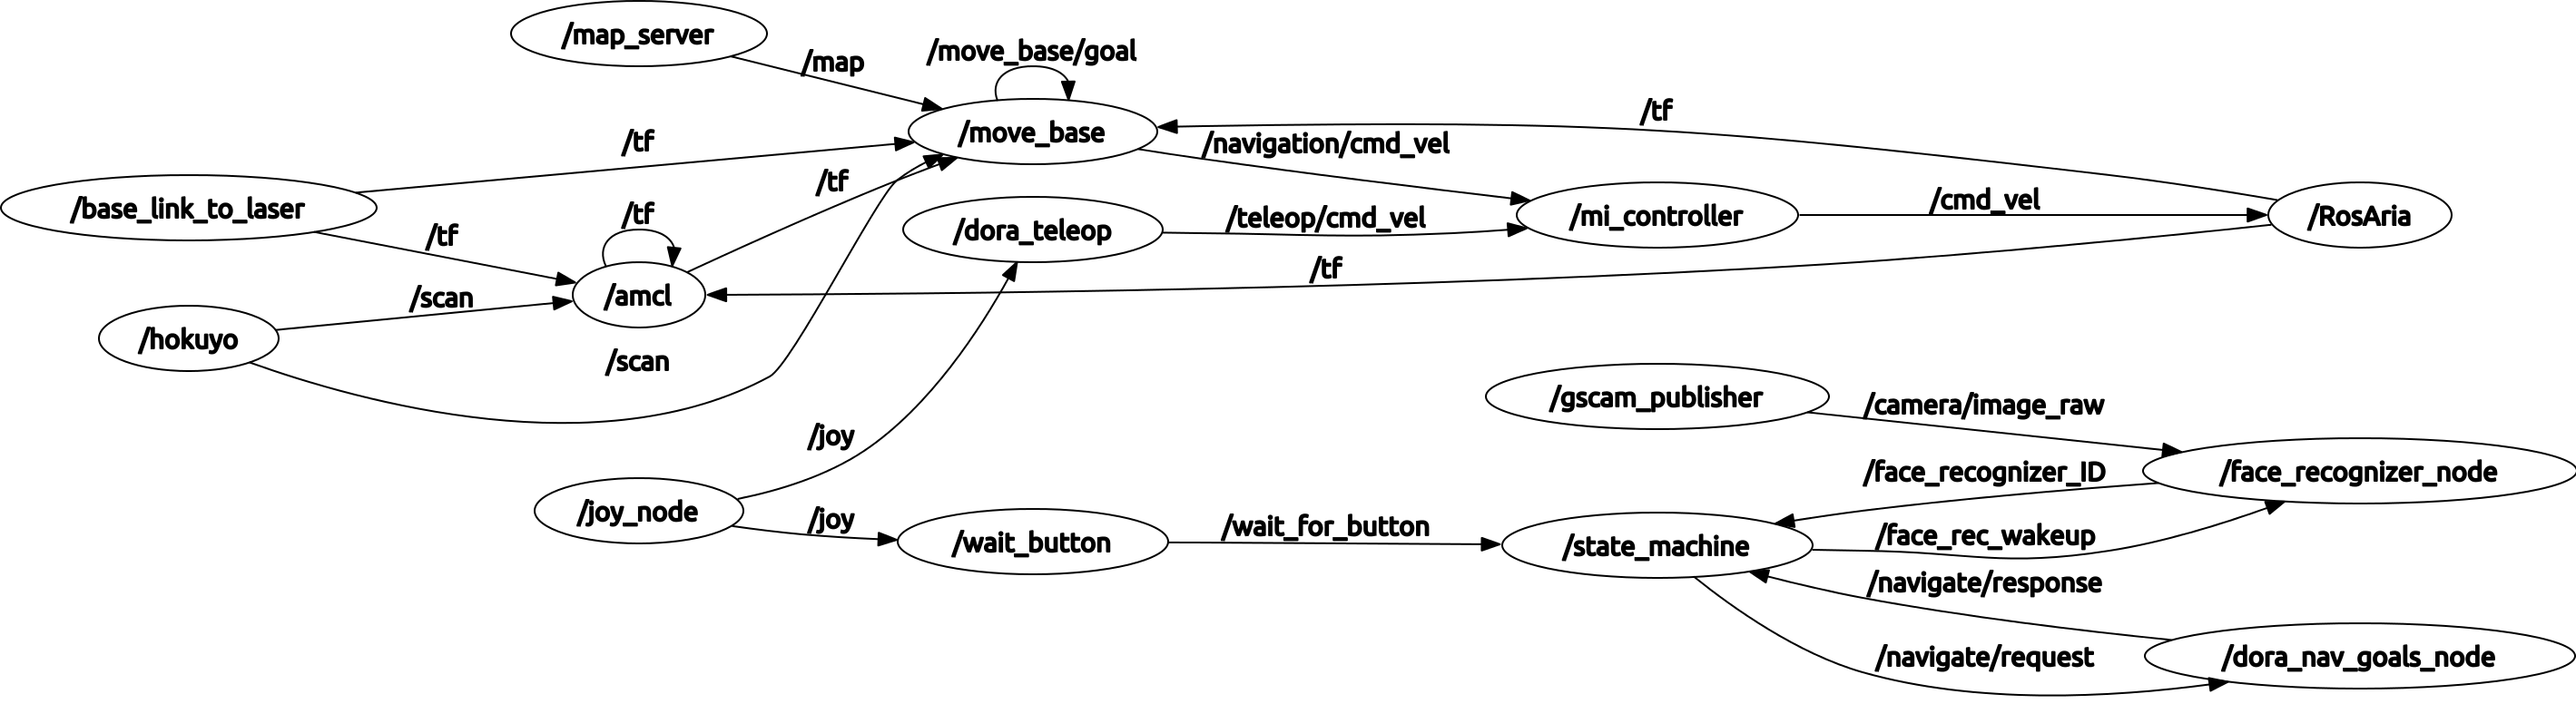
\includegraphics[width=\textwidth]{nodes_cut.png}
%\caption{An overview of the software architecture and how the nodes connect and interact with each other}
%\label{fig:nodes}
%\end{figure*}




